% Options for packages loaded elsewhere
% Options for packages loaded elsewhere
\PassOptionsToPackage{unicode}{hyperref}
\PassOptionsToPackage{hyphens}{url}
\PassOptionsToPackage{dvipsnames,svgnames,x11names}{xcolor}
%
\documentclass[
  english,
  10pt,
  letterpaper,
  DIV=11,
  numbers=noendperiod]{scrartcl}
\usepackage{xcolor}
\usepackage[margin=1in]{geometry}
\usepackage{amsmath,amssymb}
\setcounter{secnumdepth}{5}
\usepackage{iftex}
\ifPDFTeX
  \usepackage[T1]{fontenc}
  \usepackage[utf8]{inputenc}
  \usepackage{textcomp} % provide euro and other symbols
\else % if luatex or xetex
  \usepackage{unicode-math} % this also loads fontspec
  \defaultfontfeatures{Scale=MatchLowercase}
  \defaultfontfeatures[\rmfamily]{Ligatures=TeX,Scale=1}
\fi
\usepackage{lmodern}
\ifPDFTeX\else
  % xetex/luatex font selection
\fi
% Use upquote if available, for straight quotes in verbatim environments
\IfFileExists{upquote.sty}{\usepackage{upquote}}{}
\IfFileExists{microtype.sty}{% use microtype if available
  \usepackage[]{microtype}
  \UseMicrotypeSet[protrusion]{basicmath} % disable protrusion for tt fonts
}{}
\makeatletter
\@ifundefined{KOMAClassName}{% if non-KOMA class
  \IfFileExists{parskip.sty}{%
    \usepackage{parskip}
  }{% else
    \setlength{\parindent}{0pt}
    \setlength{\parskip}{6pt plus 2pt minus 1pt}}
}{% if KOMA class
  \KOMAoptions{parskip=half}}
\makeatother
% Make \paragraph and \subparagraph free-standing
\makeatletter
\ifx\paragraph\undefined\else
  \let\oldparagraph\paragraph
  \renewcommand{\paragraph}{
    \@ifstar
      \xxxParagraphStar
      \xxxParagraphNoStar
  }
  \newcommand{\xxxParagraphStar}[1]{\oldparagraph*{#1}\mbox{}}
  \newcommand{\xxxParagraphNoStar}[1]{\oldparagraph{#1}\mbox{}}
\fi
\ifx\subparagraph\undefined\else
  \let\oldsubparagraph\subparagraph
  \renewcommand{\subparagraph}{
    \@ifstar
      \xxxSubParagraphStar
      \xxxSubParagraphNoStar
  }
  \newcommand{\xxxSubParagraphStar}[1]{\oldsubparagraph*{#1}\mbox{}}
  \newcommand{\xxxSubParagraphNoStar}[1]{\oldsubparagraph{#1}\mbox{}}
\fi
\makeatother


\usepackage{longtable,booktabs,array}
\newcounter{none} % for unnumbered tables
\usepackage{calc} % for calculating minipage widths
% Correct order of tables after \paragraph or \subparagraph
\usepackage{etoolbox}
\makeatletter
\patchcmd\longtable{\par}{\if@noskipsec\mbox{}\fi\par}{}{}
\makeatother
% Allow footnotes in longtable head/foot
\IfFileExists{footnotehyper.sty}{\usepackage{footnotehyper}}{\usepackage{footnote}}
\makesavenoteenv{longtable}
\usepackage{graphicx}
\makeatletter
\newsavebox\pandoc@box
\newcommand*\pandocbounded[1]{% scales image to fit in text height/width
  \sbox\pandoc@box{#1}%
  \Gscale@div\@tempa{\textheight}{\dimexpr\ht\pandoc@box+\dp\pandoc@box\relax}%
  \Gscale@div\@tempb{\linewidth}{\wd\pandoc@box}%
  \ifdim\@tempb\p@<\@tempa\p@\let\@tempa\@tempb\fi% select the smaller of both
  \ifdim\@tempa\p@<\p@\scalebox{\@tempa}{\usebox\pandoc@box}%
  \else\usebox{\pandoc@box}%
  \fi%
}
% Set default figure placement to htbp
\def\fps@figure{htbp}
\makeatother


% definitions for citeproc citations
\NewDocumentCommand\citeproctext{}{}
\NewDocumentCommand\citeproc{mm}{%
  \begingroup\def\citeproctext{#2}\cite{#1}\endgroup}
\makeatletter
 % allow citations to break across lines
 \let\@cite@ofmt\@firstofone
 % avoid brackets around text for \cite:
 \def\@biblabel#1{}
 \def\@cite#1#2{{#1\if@tempswa , #2\fi}}
\makeatother
\newlength{\cslhangindent}
\setlength{\cslhangindent}{1.5em}
\newlength{\csllabelwidth}
\setlength{\csllabelwidth}{3em}
\newenvironment{CSLReferences}[2] % #1 hanging-indent, #2 entry-spacing
 {\begin{list}{}{%
  \setlength{\itemindent}{0pt}
  \setlength{\leftmargin}{0pt}
  \setlength{\parsep}{0pt}
  % turn on hanging indent if param 1 is 1
  \ifodd #1
   \setlength{\leftmargin}{\cslhangindent}
   \setlength{\itemindent}{-1\cslhangindent}
  \fi
  % set entry spacing
  \setlength{\itemsep}{#2\baselineskip}}}
 {\end{list}}
\usepackage{calc}
\newcommand{\CSLBlock}[1]{\hfill\break\parbox[t]{\linewidth}{\strut\ignorespaces#1\strut}}
\newcommand{\CSLLeftMargin}[1]{\parbox[t]{\csllabelwidth}{\strut#1\strut}}
\newcommand{\CSLRightInline}[1]{\parbox[t]{\linewidth - \csllabelwidth}{\strut#1\strut}}
\newcommand{\CSLIndent}[1]{\hspace{\cslhangindent}#1}

\ifLuaTeX
\usepackage[bidi=basic,shorthands=off]{babel}
\else
\usepackage[bidi=default,shorthands=off]{babel}
\fi
\ifLuaTeX
  \usepackage{selnolig} % disable illegal ligatures
\fi


\setlength{\emergencystretch}{3em} % prevent overfull lines

\providecommand{\tightlist}{%
  \setlength{\itemsep}{0pt}\setlength{\parskip}{0pt}}



 


\KOMAoption{captions}{tableheading}
\makeatletter
\@ifpackageloaded{caption}{}{\usepackage{caption}}
\AtBeginDocument{%
\ifdefined\contentsname
  \renewcommand*\contentsname{Table of contents}
\else
  \newcommand\contentsname{Table of contents}
\fi
\ifdefined\listfigurename
  \renewcommand*\listfigurename{List of Figures}
\else
  \newcommand\listfigurename{List of Figures}
\fi
\ifdefined\listtablename
  \renewcommand*\listtablename{List of Tables}
\else
  \newcommand\listtablename{List of Tables}
\fi
\ifdefined\figurename
  \renewcommand*\figurename{Figure}
\else
  \newcommand\figurename{Figure}
\fi
\ifdefined\tablename
  \renewcommand*\tablename{Table}
\else
  \newcommand\tablename{Table}
\fi
}
\@ifpackageloaded{float}{}{\usepackage{float}}
\floatstyle{ruled}
\@ifundefined{c@chapter}{\newfloat{codelisting}{h}{lop}}{\newfloat{codelisting}{h}{lop}[chapter]}
\floatname{codelisting}{Listing}
\newcommand*\listoflistings{\listof{codelisting}{List of Listings}}
\makeatother
\makeatletter
\makeatother
\makeatletter
\@ifpackageloaded{caption}{}{\usepackage{caption}}
\@ifpackageloaded{subcaption}{}{\usepackage{subcaption}}
\makeatother
\usepackage{bookmark}
\IfFileExists{xurl.sty}{\usepackage{xurl}}{} % add URL line breaks if available
\urlstyle{same}
% fallback for those not using the hyperref driver hyperxmp:
\makeatletter
\@ifundefined{xmpquote}{\newcommand{\xmpquote}[1]{#1}}{}
\makeatother
\hypersetup{
  pdftitle={What Can Be Estimated?},
  pdfauthor={Complex--Itô Random-Walk Research Project},
  pdflang={en},
  pdfkeywords={\xmpquote{stochastic
correlation}, \xmpquote{identifiability}, \xmpquote{maximum
likelihood}, \xmpquote{realized correlation}, \xmpquote{PIT
tests}, \xmpquote{attenuation}},
  colorlinks=true,
  linkcolor={blue},
  filecolor={Maroon},
  citecolor={Blue},
  urlcolor={Blue},
  pdfcreator={LaTeX via pandoc}}


\title{What Can Be Estimated?}
\usepackage{etoolbox}
\makeatletter
\providecommand{\subtitle}[1]{% add subtitle to \maketitle
  \apptocmd{\@title}{\par {\large #1 \par}}{}{}
}
\makeatother
\subtitle{Scale Observational Equivalence and Exact Maximum Likelihood
for Bounded-Factor Correlation Models}
\author{Complex--Itô Random-Walk Research Project}
\date{August 21, 2026}
\begin{document}
\maketitle
\begin{abstract}
For the bounded-factor correlation model \(\rho_t=X_t/\sqrt{X_t^2+c^2}\)
with \(dX=\mu\,dt+\sigma\,dW\) we prove a structural identifiability
theorem: the parameter triples \((c,\mu,\sigma)\) and
\((\lambda c,\mu/\lambda,\sigma/\lambda)\) induce \emph{identical} laws
for every observable correlation functional --- and, because the
Dambis--Dubins--Schwarz clock depends only on the correlation path, for
every derivative price as well. Only the ratios \(\mu/c\) and
\(\sigma/c\) exist in the identified parameter space. Estimation
therefore proceeds in the normalized coordinate
\(x=\rho/\sqrt{1-\rho^2}\), where increments are exactly Gaussian and
the exact maximum likelihood estimator of the ratio pair is ordinary
least squares --- no numerical optimization. We construct consistent
Jacobians for Fisher-space competitors (random walk;
Ornstein--Uhlenbeck), show that marginal PIT/Kolmogorov--Smirnov tests
can miss dynamic misspecification whose uniform marginal survives, and
introduce a PIT--state-correlation diagnostic that does not.
Deterministic Monte Carlo quantifies the attenuation of window-estimated
dynamics: at the standard 60-day realized-correlation window the
volatility ratio is biased down by a factor of about four. An empirical
study of four S\&P 500 pairs (2015--2026, local data store) finds vol
ratios 0.84--1.55, drift ratios statistically indistinguishable from
zero, Ornstein--Uhlenbeck AIC dominance inherited from window smoothing,
and formal out-of-sample rejection of all iid-increment models --- an
observation-scheme violation rather than a model rejection. The audited
literature calibrates this model class by stationary-density least
squares or back-transformed OLS without an identifiability analysis; the
equivalence theorem explains why free-scale likelihoods are flat and why
reported scale parameters are initialization artifacts.
\end{abstract}

\renewcommand*\contentsname{Table of contents}
{
\setcounter{tocdepth}{2}
\tableofcontents
}

\textbf{Mathematics Subject Classification (2020):} 62M99, 62F10, 91G70,
60H10.

\textbf{JEL classification:} C13, C22, G12.

\section{Introduction}\label{sec-introduction}

Stochastic-correlation models are routinely calibrated as if all their
parameters meant something. For the bounded-factor family
\(\rho_t=f(X_t)=X_t/\sqrt{X_t^2+c^2}\), \(dX=\mu\,dt+\sigma\,dW\), the
audited practice is to fit the stationary density by nonlinear least
squares (Teng et al. 2016) or to back-transform the series and run
Ornstein--Uhlenbeck regressions (Kumar et al. 2021). Neither paper asks
what the data can identify. This paper answers that question exactly,
and the answer changes both the estimator and the interpretation.

Contributions:

\begin{enumerate}
\def\labelenumi{\arabic{enumi}.}
\tightlist
\item
  \textbf{Theorem (scale observational equivalence)}
  (Section~\ref{sec-theorem}):
  \((c,\mu,\sigma)\sim(\lambda c,\mu/\lambda,\sigma/\lambda)\) are
  indistinguishable from correlation observations \emph{and from
  derivative prices}; the identified space is two-dimensional.
\item
  \textbf{Closed-form exact MLE} of the identified pair
  (Section~\ref{sec-mle}): OLS in the normalized conjugate coordinate,
  with the consistency Jacobian that makes information criteria
  comparable across transforms.
\item
  \textbf{Conditional-uniformity diagnostics}
  (Section~\ref{sec-diagnostics}): marginal PIT/KS misses dynamic
  misspecification whose \(u\)-marginal stays nearly uniform;
  correlating PIT values with the lagged state detects it at eight
  standard errors where KS has no power (\(p=0.53\)).
\item
  \textbf{Attenuation law} (Section~\ref{sec-attenuation}):
  deterministic Monte Carlo shows window-smoothed proxies damp measured
  dynamics \textasciitilde4× at the standard 60-day choice.
\item
  \textbf{Empirics} (Section~\ref{sec-empirics}): four liquid pairs,
  exact estimation, honest out-of-sample verdicts.
\end{enumerate}

\section{The equivalence theorem}\label{sec-theorem}

\textbf{Theorem (scale observational equivalence).} \emph{For every
\(\lambda>0\) the parameter triples \((c,\mu,\sigma)\) and
\((\lambda c,\mu/\lambda,\sigma/\lambda)\) generate identical laws for}

\[
(\rho_{t_1},\dots,\rho_{t_n})\quad\text{for every finite } n
\text{ and every } t_1<\dots<t_n .
\]

\emph{Consequently they also generate identical laws for every
functional of the correlation path --- including occupation integrals
\(A_T=\int_0^T\rho_sds\) and hence every spread/basket derivative
price.}

\emph{Proof sketch.} With \(Y=X/c\), \(\rho=F(Y)\) for the
parameter-free map \(F(y)=y/\sqrt{y^2+1}\), and \(Y\) is drifted
Brownian motion with drift \(\mu/c\) and volatility \(\sigma/c\). Every
observable is a functional of the \(Y\)-path alone. ∎

Three consequences:

\begin{itemize}
\tightlist
\item
  \textbf{No free-scale likelihoods.} The profile likelihood in \(c\) is
  exactly flat; any reported ``MLE of \(c\)'' from correlation data
  alone is an artifact of optimizer initialization. (We observed this
  numerically before deriving the theorem.)
\item
  \textbf{Prices do not rescue identification}: the DDS clock
  \(v=\beta T+\alpha A_T\) is itself a path functional.
\item
  \textbf{Exogenous time rulers break the degeneracy}: if
  \(\sigma(\cdot)\) is known exogenously (as in the pricing calibration
  of the term-structure paper), \(\lambda^{\mathbb Q}\) re-emerges as
  identified.
\end{itemize}

\section{Closed-form exact MLE}\label{sec-mle}

Work in the normalized coordinate \(x=g(\rho)=\rho/\sqrt{1-\rho^2}\).
Under exact-skeleton observation,

\[
\Delta x_i \sim N\!\Big(\tfrac{\mu}{c}\Delta t,\ (\tfrac{\sigma}{c})^2\Delta t\Big),
\]

so the exact MLE of the identified pair is the OLS solution --- mean and
root-mean-square of increments --- plus the Jacobian of the observation
map, \(\log|dx/d\rho|=-\tfrac{3}{2}\log(1-\rho^2)\) summed over
transitions. Competitors receive the same treatment with their own
Jacobians: Fisher random walk (\(y=\operatorname{atanh}\rho\)) and
Fisher OU (exact AR(1) quasi-MLE, profiled over the reversion speed).
Verification: ratio recovery within Monte Carlo tolerance on synthetic
skeletons; likelihood invariance under rescaling; information criteria
rank the generating model.

\section{Diagnostics}\label{sec-diagnostics}

One-step-ahead PIT values \(u_i=P(\rho_i\le\text{obs}\mid\rho_{i-1})\)
are exact under each fitted model's transition law. Two complementary
checks:

\begin{itemize}
\tightlist
\item
  \textbf{Marginal KS} against Uniform(0,1) --- calibration;
\item
  \textbf{PIT--state correlation} --- dynamic adequacy. Fitting a random
  walk to genuinely mean-reverting data produces \(u\)-marginals that
  stay near uniform (KS \(p=0.53\) in our experiment) while
  \(\operatorname{corr}(u,y_{\text{prev}})=-0.148\approx8\) standard
  errors. Marginal KS alone would certify a wrong model.
\end{itemize}

\section{Attenuation}\label{sec-attenuation}

Realized correlations are window estimates, not skeleton observations.
Simulating the true latent system, forming rolling correlations, and
refitting gives the attenuation factor of the volatility ratio:

{\def\LTcaptype{none} % do not increment counter
\begin{longtable}[]{@{}lll@{}}
\toprule\noalign{}
window (days) & est./true vol ratio & IQR \\
\midrule\noalign{}
\endhead
\bottomrule\noalign{}
\endlastfoot
20 & 1.209 & 0.219 \\
40 & 0.379 & 0.072 \\
60 & 0.253 & 0.043 \\
120 & 0.077 & 0.015 \\
\end{longtable}
}

At the market-standard 60-day choice the measured dynamics are damped
\textasciitilde4×; short windows can even inflate them. Any calibration
quoted from smoothed proxies must invert this curve first
(Figure~\ref{fig-attenuation}).

\begin{figure}[tbp]

\centering{

\pandocbounded{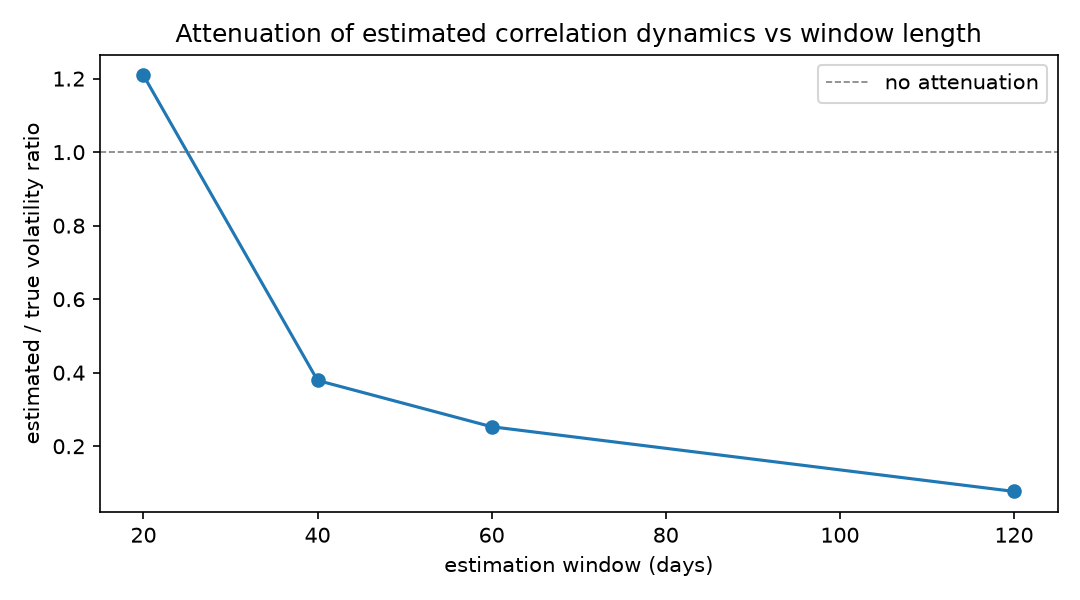
\includegraphics[keepaspectratio]{figures/phase9_attenuation.png}}

}

\caption{\label{fig-attenuation}Attenuation factor vs estimation window
(deterministic MC, 24 replications per cell).}

\end{figure}%

\section{Empirical study}\label{sec-empirics}

Data: daily adjusted closes 2015-01-01 → 2026-08-14 from a local store;
60-day rolling Pearson correlations (2,860 windows per pair)
(\textbf{?@fig-series}).

{\def\LTcaptype{none} % do not increment counter
\begin{longtable}[]{@{}lllll@{}}
\toprule\noalign{}
pair & mean \(\rho\) & sd & est. \(\mu/c\) & est. \(\sigma/c\) \\
\midrule\noalign{}
\endhead
\bottomrule\noalign{}
\endlastfoot
XOM/CVX & +0.793 & 0.123 & −0.020 & 1.169 \\
JPM/BAC & +0.847 & 0.099 & +0.017 & 1.552 \\
KO/PEP & +0.700 & 0.120 & −0.009 & 0.913 \\
AAPL/MSFT & +0.550 & 0.223 & −0.032 & 0.841 \\
\end{longtable}
}

Drift ratios are statistically zero (SE ≈ 0.11/yr at these sample
sizes). Fisher-OU wins AIC everywhere but with weak reversion
(\(\kappa\approx1.4\)--2.3/yr) --- persistence largely inherited from
overlapping windows. Out-of-sample (70/30 split), \emph{all}
iid-increment models are rejected by marginal KS --- expected, since
smoothed proxies violate the exact-skeleton scheme --- while the
state-correlation diagnostic separates structures: RW-type fits show
\(z\) down to −2.6, the OU stays within ±1.2. Log-score ranking follows
the smoothing artifact, not the latent truth; we report it as such.

\begin{figure}[tbp]

\centering{

\pandocbounded{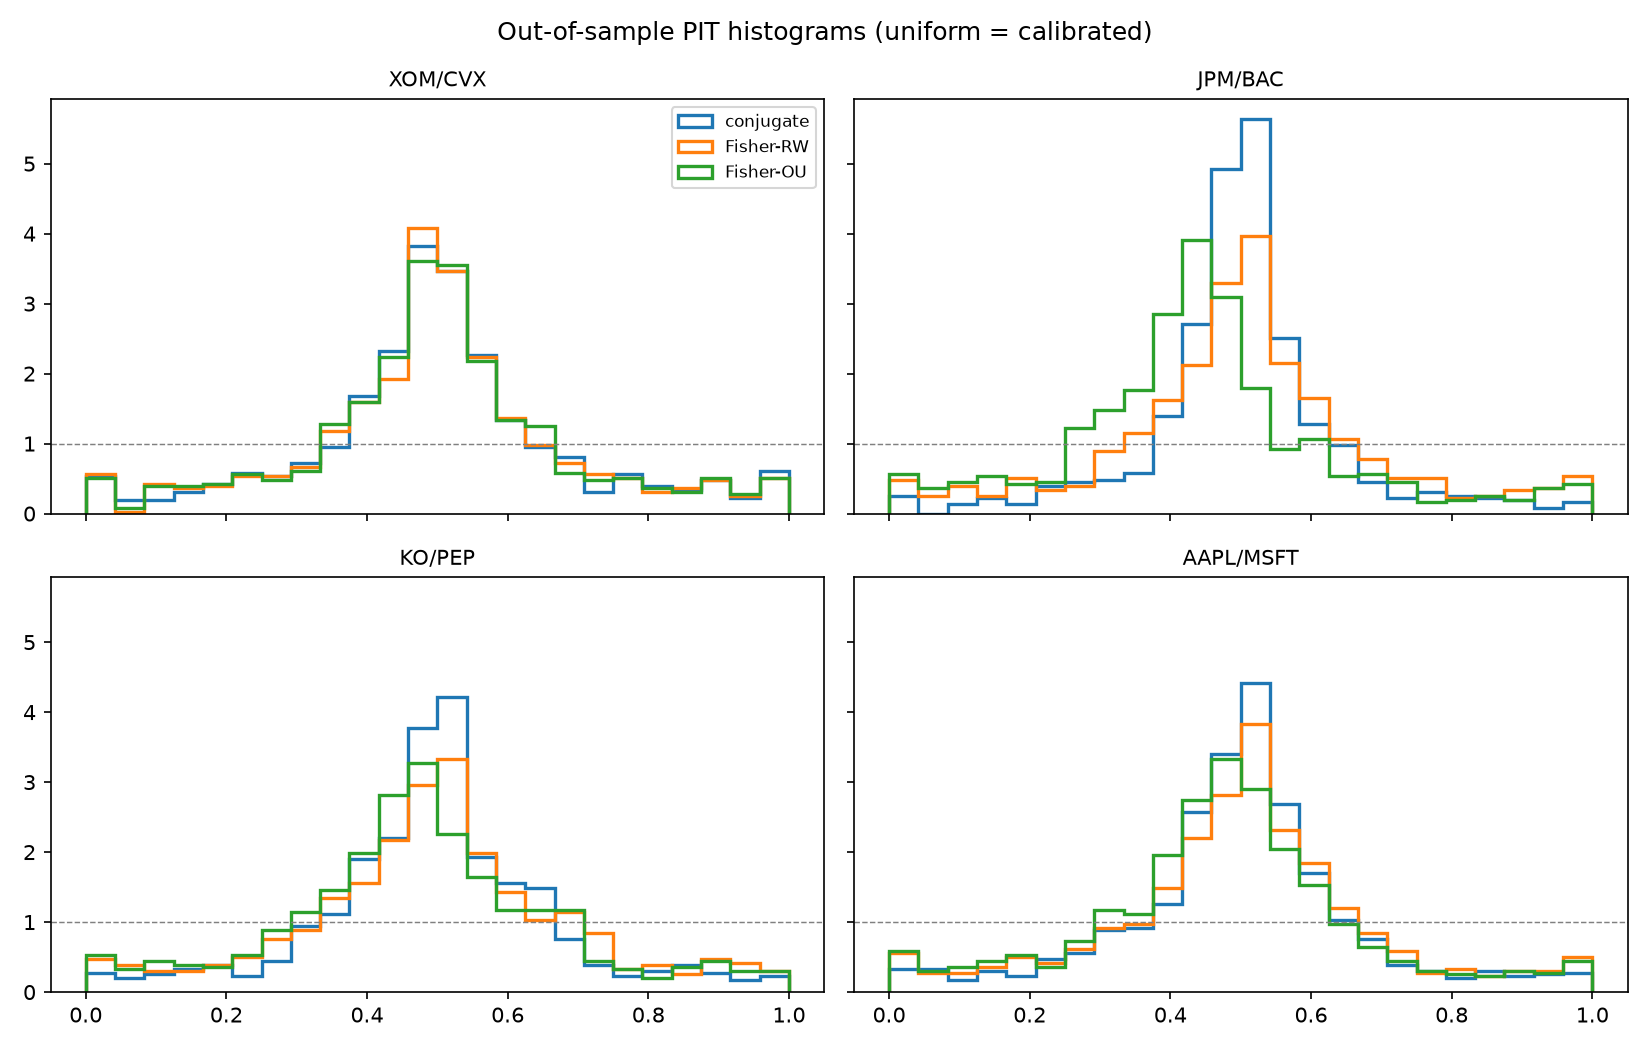
\includegraphics[keepaspectratio]{figures/phase9_pit_histograms.png}}

}

\caption{\label{fig-pit}Out-of-sample PIT histograms by pair and model.}

\end{figure}%

\section{Related literature}\label{sec-related}

Identifiability analyses are standard for stochastic volatility
(Aït-Sahalia--Kimmel lineage) but absent for bounded correlation
factors; Teng et al. (2016) explicitly call the likelihood ``tedious''
and fit stationary densities instead; Kumar et al. (2021) use
back-transformed least squares; Aas et al. (2010) estimate dynamic
copulas by efficient importance sampling. None states an equivalence
theorem; none provides closed-form exact MLE; none quantifies proxy
attenuation for this class. Realized-volatility proxy methodology
(Barndorff-Nielsen and Shephard 2002) supplies the conceptual template
we adapt.

\section{Conclusion}\label{sec-conclusion}

Two parameters exist; one equation each estimates them exactly; one
extra diagnostic guards against the failure mode that marginal tests
miss; and one curve converts quoted calibrations into latent-truth
statements. That is the entire estimation content of the bounded-factor
model --- and it is fully explicit.

\section{Reproducibility}\label{sec-repro}

Environment: conda \texttt{phase3-paper} (Python 3.12.13, numpy 2.5.1,
pandas, scipy 1.18.0). Notebook
\texttt{notebooks/phase9\_estimation\_empirical.ipynb} (\textasciitilde6
s, seed 20260821); module \texttt{phase9\_estimation.py}; tests
\texttt{tests/test\_phase9\_estimation.py} (14/14). Data read from the
local alpha-engine store (\texttt{prices/*.parquet}, adjusted closes).

\protect\phantomsection\label{refs}
\begin{CSLReferences}{1}{1}
\bibitem[\citeproctext]{ref-aas2010}
Aas, Kjersti, Claudia Czado, Arnoldo Frigessi, and Henrik Bakken. 2010.
{``Dynamic Stochastic Copula Models: Estimation, Inference and
Applications.''} \emph{Journal of Applied Econometrics} 25 (2):
289--315.

\bibitem[\citeproctext]{ref-barnsdorff2002}
Barndorff-Nielsen, Ole E., and Neil Shephard. 2002. {``Econometric
Analysis of Realised Volatility and Its Use in Estimating Stochastic
Volatility Models.''} \emph{Journal of the Royal Statistical Society B}
64 (2): 253--80.

\bibitem[\citeproctext]{ref-kumar2021}
Kumar, Ashish, László Márkus, and Norbert Hári. 2021.
\emph{Arbitrage-Free Pricing of {CVA} for Cross-Currency Swap with
Wrong-Way Risk Under Stochastic Correlation Modeling Framework}.

\bibitem[\citeproctext]{ref-teng2016}
Teng, Long, Matthias Ehrhardt, and Michael Günther. 2016. {``Modelling
Stochastic Correlation.''} \emph{Journal of Mathematics in Industry} 6
(1): 1--18. \url{https://doi.org/10.1186/s13362-016-0018-4}.

\end{CSLReferences}




\end{document}
